\section[AGC]{Automatiskt förstärkningsreglering (AGC)}
\textbf{HAREC a.\ref{HAREC.a.4.3.8}\label{myHAREC.a.4.3.8}}
\index{automatisk förstärkningreglering}
\index{AGC}
\index{mottagare!automatisk förstärkningsreglering}
\index{mottagare!AGC}

För att mottagaren ska fungera bra för såväl mycket svaga som för mycket starka
insignaler behövs en förstärkningsreglering i signalvägen genom mottagaren.
Signalspänningen på mottagaringången kan vara från delar av en mikrovolt upp
till över 100~millivolt -- ett spänningsförhållande på 1:100 000.
Det motsvarar mer än nio S-enheter, vilket är ett mått på signalstyrkan
(se bilaga \ref{s-enhet}).

Vid mottagning av en stark signal är det inte tillräckligt med att
bara minska LF-förstärkningen.
Förstärkarstegen i HF- och MF-delen blir ändå överstyrda av den starka
insignalen och utsignalen förvrängs om inget ytterligare görs.
Det är därför nödvändigt att minska förstärkningen även i HF- och
MF-förstärkarstegen, ju mer desto starkare insignalen är.
Som hjälpmedel finns oftast ett reglage för HF-förstärkningen (RF gain), och
därutöver en \emph{automatisk förstärkningsreglering} (eng. \emph{Automatic Gain Control (AGC)}).

En mottagare med god reglering kan arbeta med signalstyrkor mellan mikrovolt
och volt.
Beroende hur den mottagna signalen är modulerad (sändningsslaget), sker AGC
på olika sätt.

Både vid AM och SSB finns informationen i sidbanden.
HF- och MF-stegen måste därför arbeta i det linjära området och de får inte
överstyras.
Förstärkningen i mottagaren måste alltså regleras med hänsyn till detta.

\subsection{AGC vid AM (A3E)}
\index{amplitudmodulation}
\index{AGC}
\index{A3E}

\begin{figure}
  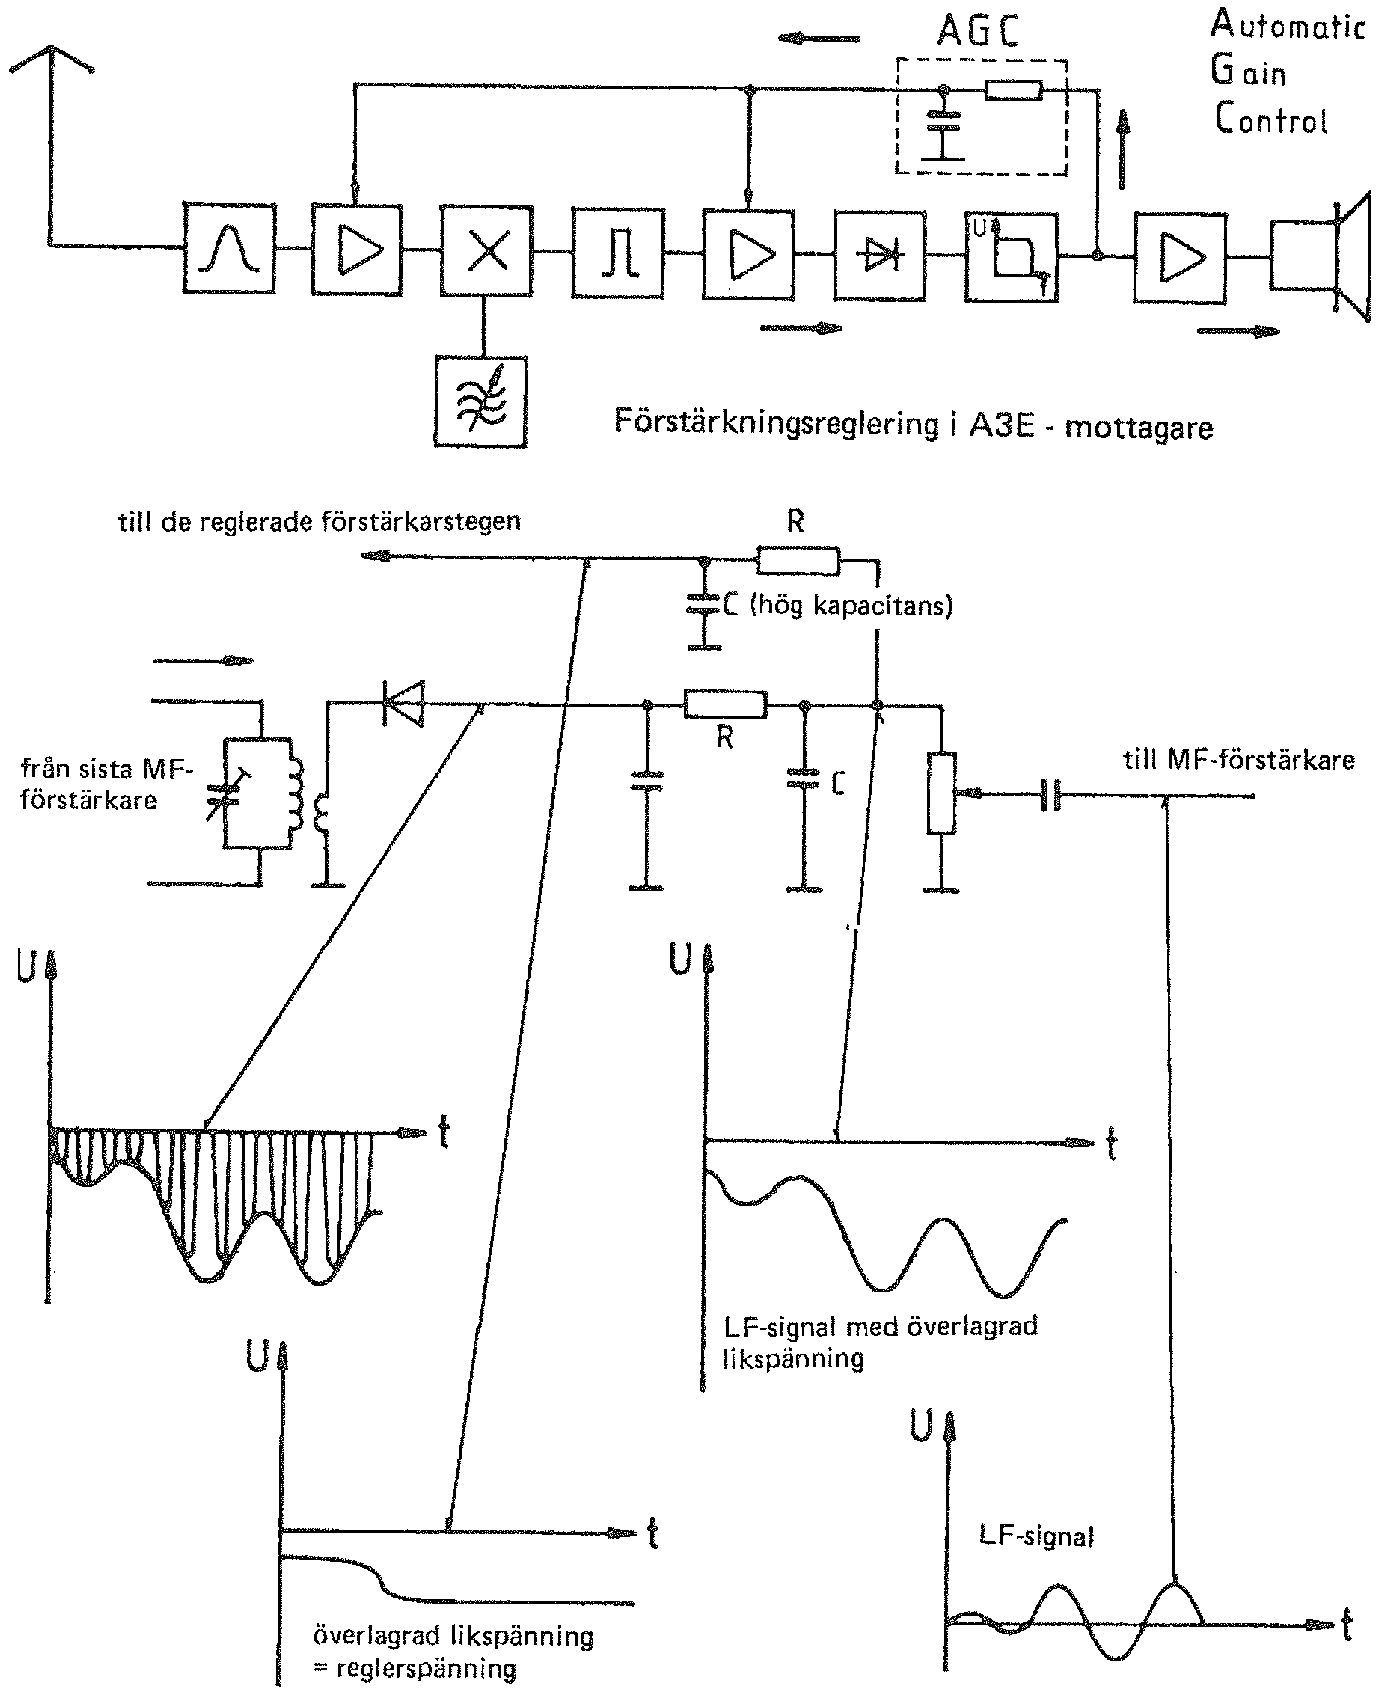
\includegraphics[width=\textwidth]{images/cropped_pdfs/bild_2_4-20.pdf}
  \caption{AGC vid AM-mottagning med superheterodynmottagare}
  \label{fig:bildII4-20}
\end{figure}

Den likspänning som uppstår vid demoduleringen av MF-signalen i en
AM-mottagare används till förstärkningsreglering -- AGC, så som illustreras
i bild \ref{fig:bildII4-20}.
Den LF-spänning som är överlagrad på likspänningen undertrycks i ett
RC-lågpassfilter.
Likspänningen över kondensatorn följer variationerna i den mottagna signalens
styrka med en tidskonstant av ca 0,1~sekunder.
Likspänningen blir alltså inte påverkad av de betydligt snabbare
spänningsändringarna som kommer av moduleringen.

En stark bärvågssignal alstrar en hög likspänning och en svag signal
en låg likspänning, oberoende av moduleringen.
Denna likspänning återförs till de framförliggande HF- och MF-förstärkarstegen,
vilka är gjorda så att en hög reglerspänning sänker förstärkningen, medan en
låg spänning tillåter en hög förstärkning.

På så sätt kommer signalstyrkan efter de reglerade stegen att hållas
konstant samtidigt som mottagarens ingång inte överstyrs.

Den likspänning som filtrerats fram från detektorn kallas reglerspänning eller
AGC-spänning.
Diodens polarisering är inte viktig för att få ut LF vid demoduleringen, men
däremot för att få rätt polaritet på AGC-spänningen.
I de flesta mottagare används negativ AGC-spänning.

\subsection{AGC vid SSB (J3E)}
\index{SSB}
\index{AGC}

I de flesta utföranden lämnar produktdetektorn en växelspänning utan
överlagrad likspänning.
Reglerspänningen alstras därför genom likriktning av MF-spänningen med hjälp
av en separat demoduleringsdiod eller genom likriktning av LF-växelspänningen,
så som illustreras i bild \ref{fig:bildII4-21}.

Vid SSB alstras det ju ingen MF-spänning under talpauserna, eftersom
ingen bärvåg tas emot då.
Tidskonstanten på lågpassfiltret för reglerspänningen måste därför vara längre
än vid AM, d.v.s. 0,5 till 2~sekunder.
En alltför snabb tillbakagång i reglerspänningen p.g.a. en för kort
tidskonstant skulle leda till mer mottagningsbrus i talpauserna.
I moderna mottagare finns det ofta en omkopplare eller justering för olika
tidskonstanter.

\subsection{AGC vid CW (A1A)}
\index{CW}
\index{AGC}

Metoden för att alstra AGC-spänning är samma vid CW och SSB.

\subsection{AGC vid FM (F3E)}
\index{frekvensmodulation}
\index{AGC}

FM-mottagare brukar inte regleras av den anledningen att det vid FM
inte finns någon information i signalamplituden, utan finns i stället
i frekvensvariationerna i signalen.

\begin{figure}
  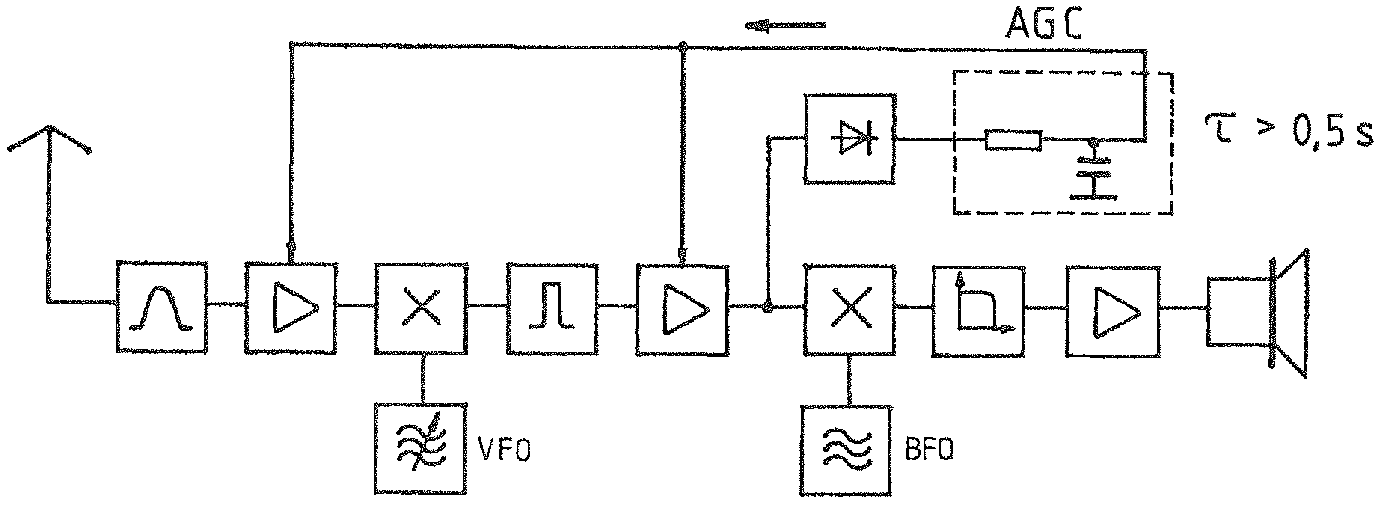
\includegraphics[width=\textwidth]{images/cropped_pdfs/bild_2_4-21.pdf}
  \caption{AGC vid SSB- och CW-mottagning med superheterodynmottagare}
  \label{fig:bildII4-21}
\end{figure}

Helt avsiktligt läggs därför förstärkningen i mottagaren så, att en
sinussignal blir en kantvåg p.g.a. överstyrning i förstärkarstegen.
Ett eller flera sådana amplitudbegränsande steg, även kallat ''limiter'',
placeras före demoduleringssteget.
Störningar av amplitudvariationer kommer då att klippas bort och inte störa
mottagningen.

Störande signaler inom nyttobandbredden har dock ingen större inverkan
så länge som den önskade signalens styrka är en halv s-enhet större än
den störande signalens styrka.
Likaså försvinner det störande bruset vid mottagning av en FM-sändare mycket
snabbt över denna signalnivå.
Amplitudmodulerade störningar, som t.ex. de från tändgnistor i
förbränningsmotorer, har liten påverkan vid tillräckligt stark nyttosignal.

\subsection{Signalstyrkemätare (S-meter)}
\textbf{HAREC a.\ref{HAREC.a.4.3.9}\label{myHAREC.a.4.3.9}}
\index{signalstyrkemätare}
\index{mottagare!signalstyrkemätare}
\index{S-meter}
\index{mottagare!S-meter}

AGC-spänningen i en mottagare för AM, CW och SSB kan även styra en
S-meter, som ger besked om hur stark signalen in i mottagaren är.
(Se bilaga \ref{s-enhet}.)

\subsection{Brusspärr}
\textbf{HAREC a.\ref{HAREC.a.4.3.10}\label{myHAREC.a.4.3.10}}
\index{brusspärr}
\index{mottagare!brusspärr}
\index{squelch}
\index{mottagare!squelch}
\index{repeater}
\index{bärvågsstyrd}

I en FM-mottagare hörs bara brus när det inte kommer in en tillräckligt stark
signal.
Bruset är genomträngande eftersom FM-mottagare arbetar med hög förstärkning.
En \emph{brusspärr} (eng. \emph{squelch}) är en anordning som stoppar
signalerna till LF-förstärkaren när signalerna ej uppnår en viss nivå.
På så sätt slipper man att höra på bruset.
I mottagare för flera sändningsslag och därför även AGC kan denna funktion
styra brusspärren, men i en ren FM-mottagare arbetar MF-förstärkarna utan AGC.
I det fallet behövs någon annan anordning för att skilja mellan en modulerad
signal och brus.
Ofta finns ett reglage (squelch) för hur stark signalen ska vara innan spärren
öppnar.

För en \emph{repeater} används brusspärren även för att starta sändaren när den
är \emph{bärvågsstyrd}, dvs. man låter signalstyrkan på den mottagna signalen
slå på även sändaren om den inkomna signalen är tillräckligt stark.
Nuförtiden anses bärvågsstyrd repeater inte lämplig, då den kan okynnesöppna av
störningar, varvid störningen förstärks.
Istället bör tonöppning eller subton användas.

\subsection{Tonöppning}
\index{tonöppning}
\index{1750 Hz}

Ett alternativ till bärvågsbaserad brusspärr är \emph{tonöppning} (eng.
\emph{1750 Hz tone-burst}) som i allmänhet är att man lägger ut en 1750 Hz
tonskur för att öppna en repeater.
En del äldre amatörer har lärt sig att vissla rätt ton för att öpnna repeatern
då de en gång i tiden inte hade handapparater med inbyggd 1750 Hz knapp.

\subsection{Subton}
\index{subton}
\index{CTCSS}

Ett problem med 1750 Hz tonöppning är när närliggande repeatrar med samma in
och utfrekvens har sådana konventioner att bägge hör handapparatens öppningston,
då kommer bägge repeatrarna riskera öppna och då störa varandras sändning.

Ett alternativ är därför att använda \emph{subton} (eng. \emph{subtone}) som är
en frekvens under 300 Hz, i allmänhet 60 till 250 Hz.
Ett existerande subton-system är \emph{Continuous Tone Coded Squelch System
  (CTCSS)} där sändaren lägger ut en kontinurlig subton.
Mottagaren detekterar en vald subton, och enbart när den tonen har tillräcklig
styrka så öppnar squelchen och håller den öppen så länge som det finns en
subton.

För repeatrar så används det för att även starta sändaren, så därför måste man
välja den subton som repeaterns mottagare är inställd på för att öppna
repeatern.
Det förekommer också att repeatern i sin tur skickar ut subton, oftast den som
används för att öppna den.
Detta öppnar i sin tur handapparaterna för den valda repeatern.
Detta kan också användas av handapparater för att hitta repeatrar och lära sig
den subton som öppnar den.

Skulle flera repeatrar höra samma källa så kan därför olika subton användas
för att undvika öppning av fel repeater.
SSA:s repeateransvarig har tilldelat CTCSS subtoner för de olika regionerna,
och inom varje region finns flera subtoner för att kunna separera inom
regionen.

\subsection{DTMF}
\index{DTMF}

Ett system för att skicka styrkommandon och även öppna repeatrar är
\emph{Dual Tone Multi Frequency (DTMF)}, som bygger på principen att man
skickar två samtidiga toner.
De två tonerna väljs som en av fyra i två olika serier.
Detta ger 4x4=16 kombinationer, varav 10 representerar siffrorna 0-9.
DTMF kommer ursprungligen från telefonisystem, men fungerar även bra över
vanliga radiokanaler.
DTMF kan användas för att styra repeatrar, som att slå på och stänga av dem,
samt styra andra egenskaper.
